\documentclass[a4paper,12pt]{article}
\usepackage{graphicx}
\usepackage{listings}
\usepackage{xcolor}

\title{Arduino 3 LED On/Off Project}
\author{Alireza Naderinasab}
\date{\today}

\begin{document}
	\maketitle
	
	\section{Project Description}
	This project demonstrates sequential control of three LEDs using Arduino.
	Each LED turns ON and OFF one after another with a 1-second delay.
	This is a basic introduction to digital output control.
	
	\section{Code}
	\begin{lstlisting}[language=C++]
		int ledPin_1 = 11;
		int ledPin_2 = 12;
		int ledPin_3 = 13;
		
		void setup(){
			pinMode(ledPin_1, OUTPUT);
			pinMode(ledPin_2, OUTPUT);
			pinMode(ledPin_3, OUTPUT);
		}
		
		void loop(){
			digitalWrite(ledPin_1, HIGH);
			delay(1000);
			digitalWrite(ledPin_1, LOW);
			delay(1000);
			
			digitalWrite(ledPin_2, HIGH);
			delay(1000);
			digitalWrite(ledPin_2, LOW);
			delay(1000);
			
			digitalWrite(ledPin_3, HIGH);
			delay(1000);
			digitalWrite(ledPin_3, LOW);
			delay(1000);
		}
	\end{lstlisting}
	
	\section{Hardware Setup}
	\begin{itemize}
		\item Arduino board
		\item 3 LEDs
		\item 3 resistors (100$\Omega$)
		\item Breadboard and wires
	\end{itemize}
	
	\section{Output Images}
	
	\subsection{LED 1}
	\begin{center}
		\includegraphics[width=0.6\textwidth]{images/img-1.jpg}
	\end{center}
	
	\subsection{LED 2}
	\begin{center}
		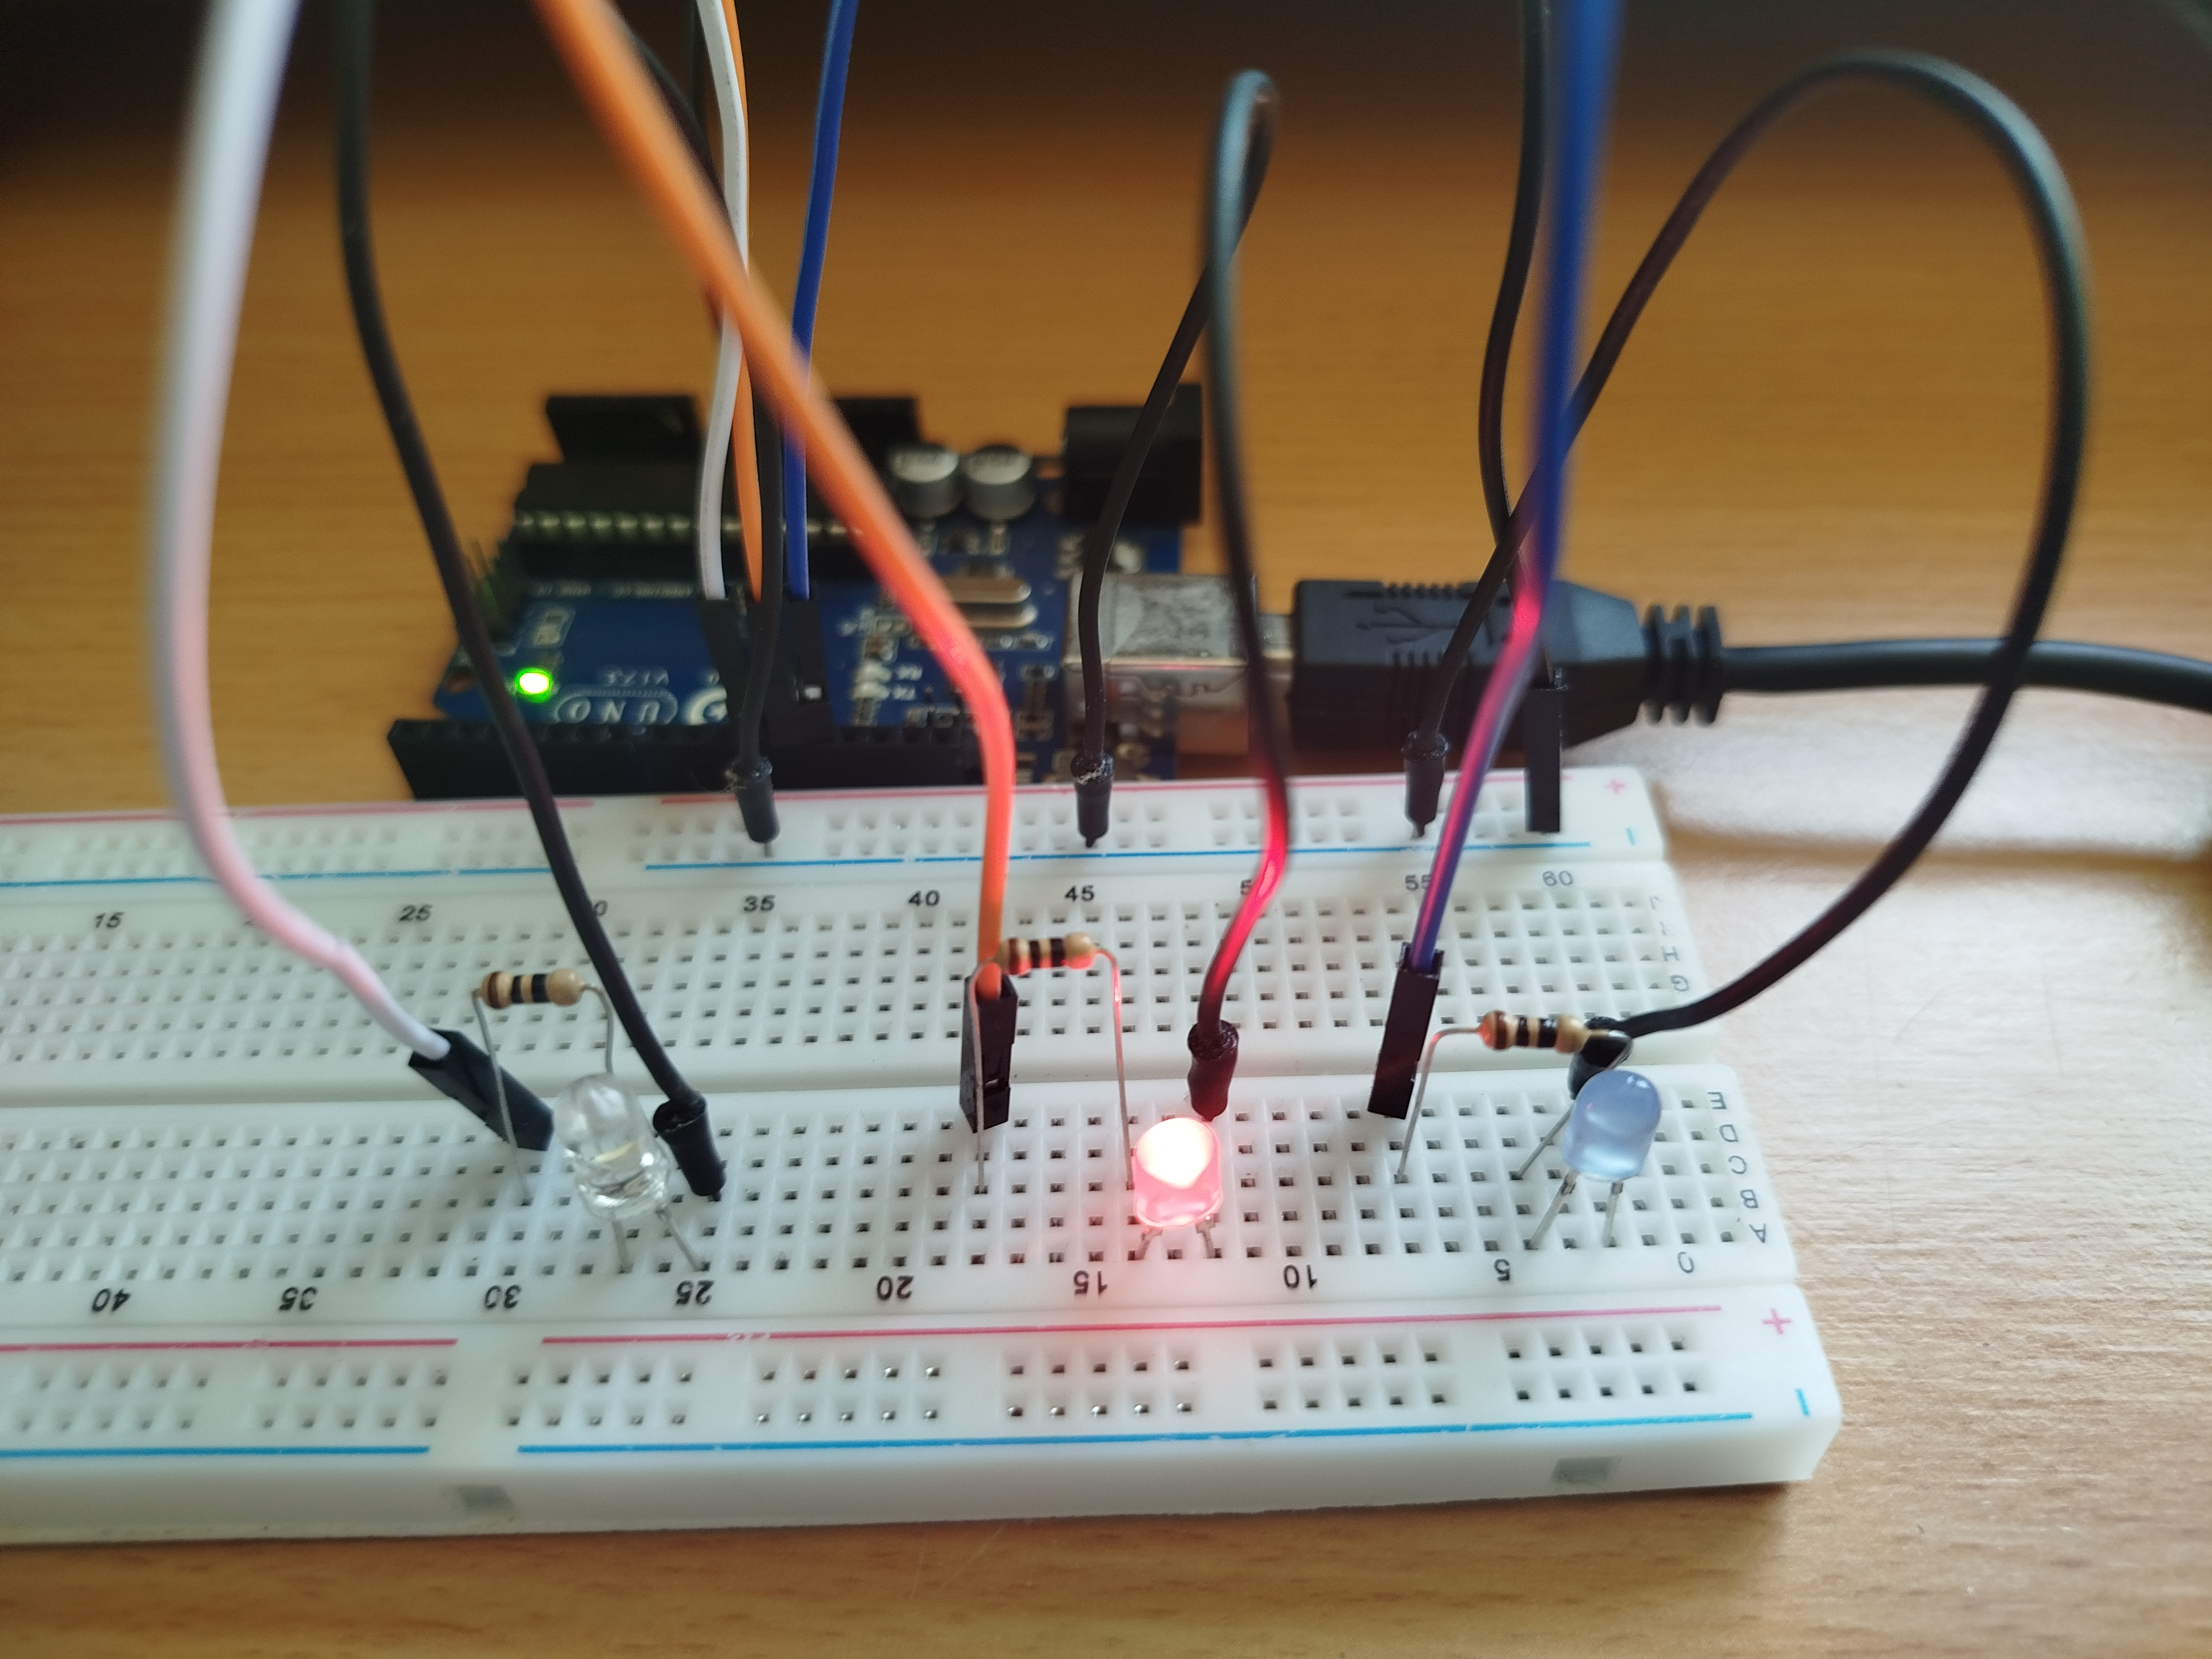
\includegraphics[width=0.6\textwidth]{images/img-2.jpg}
	\end{center}
	
	\subsection{LED 3}
	\begin{center}
		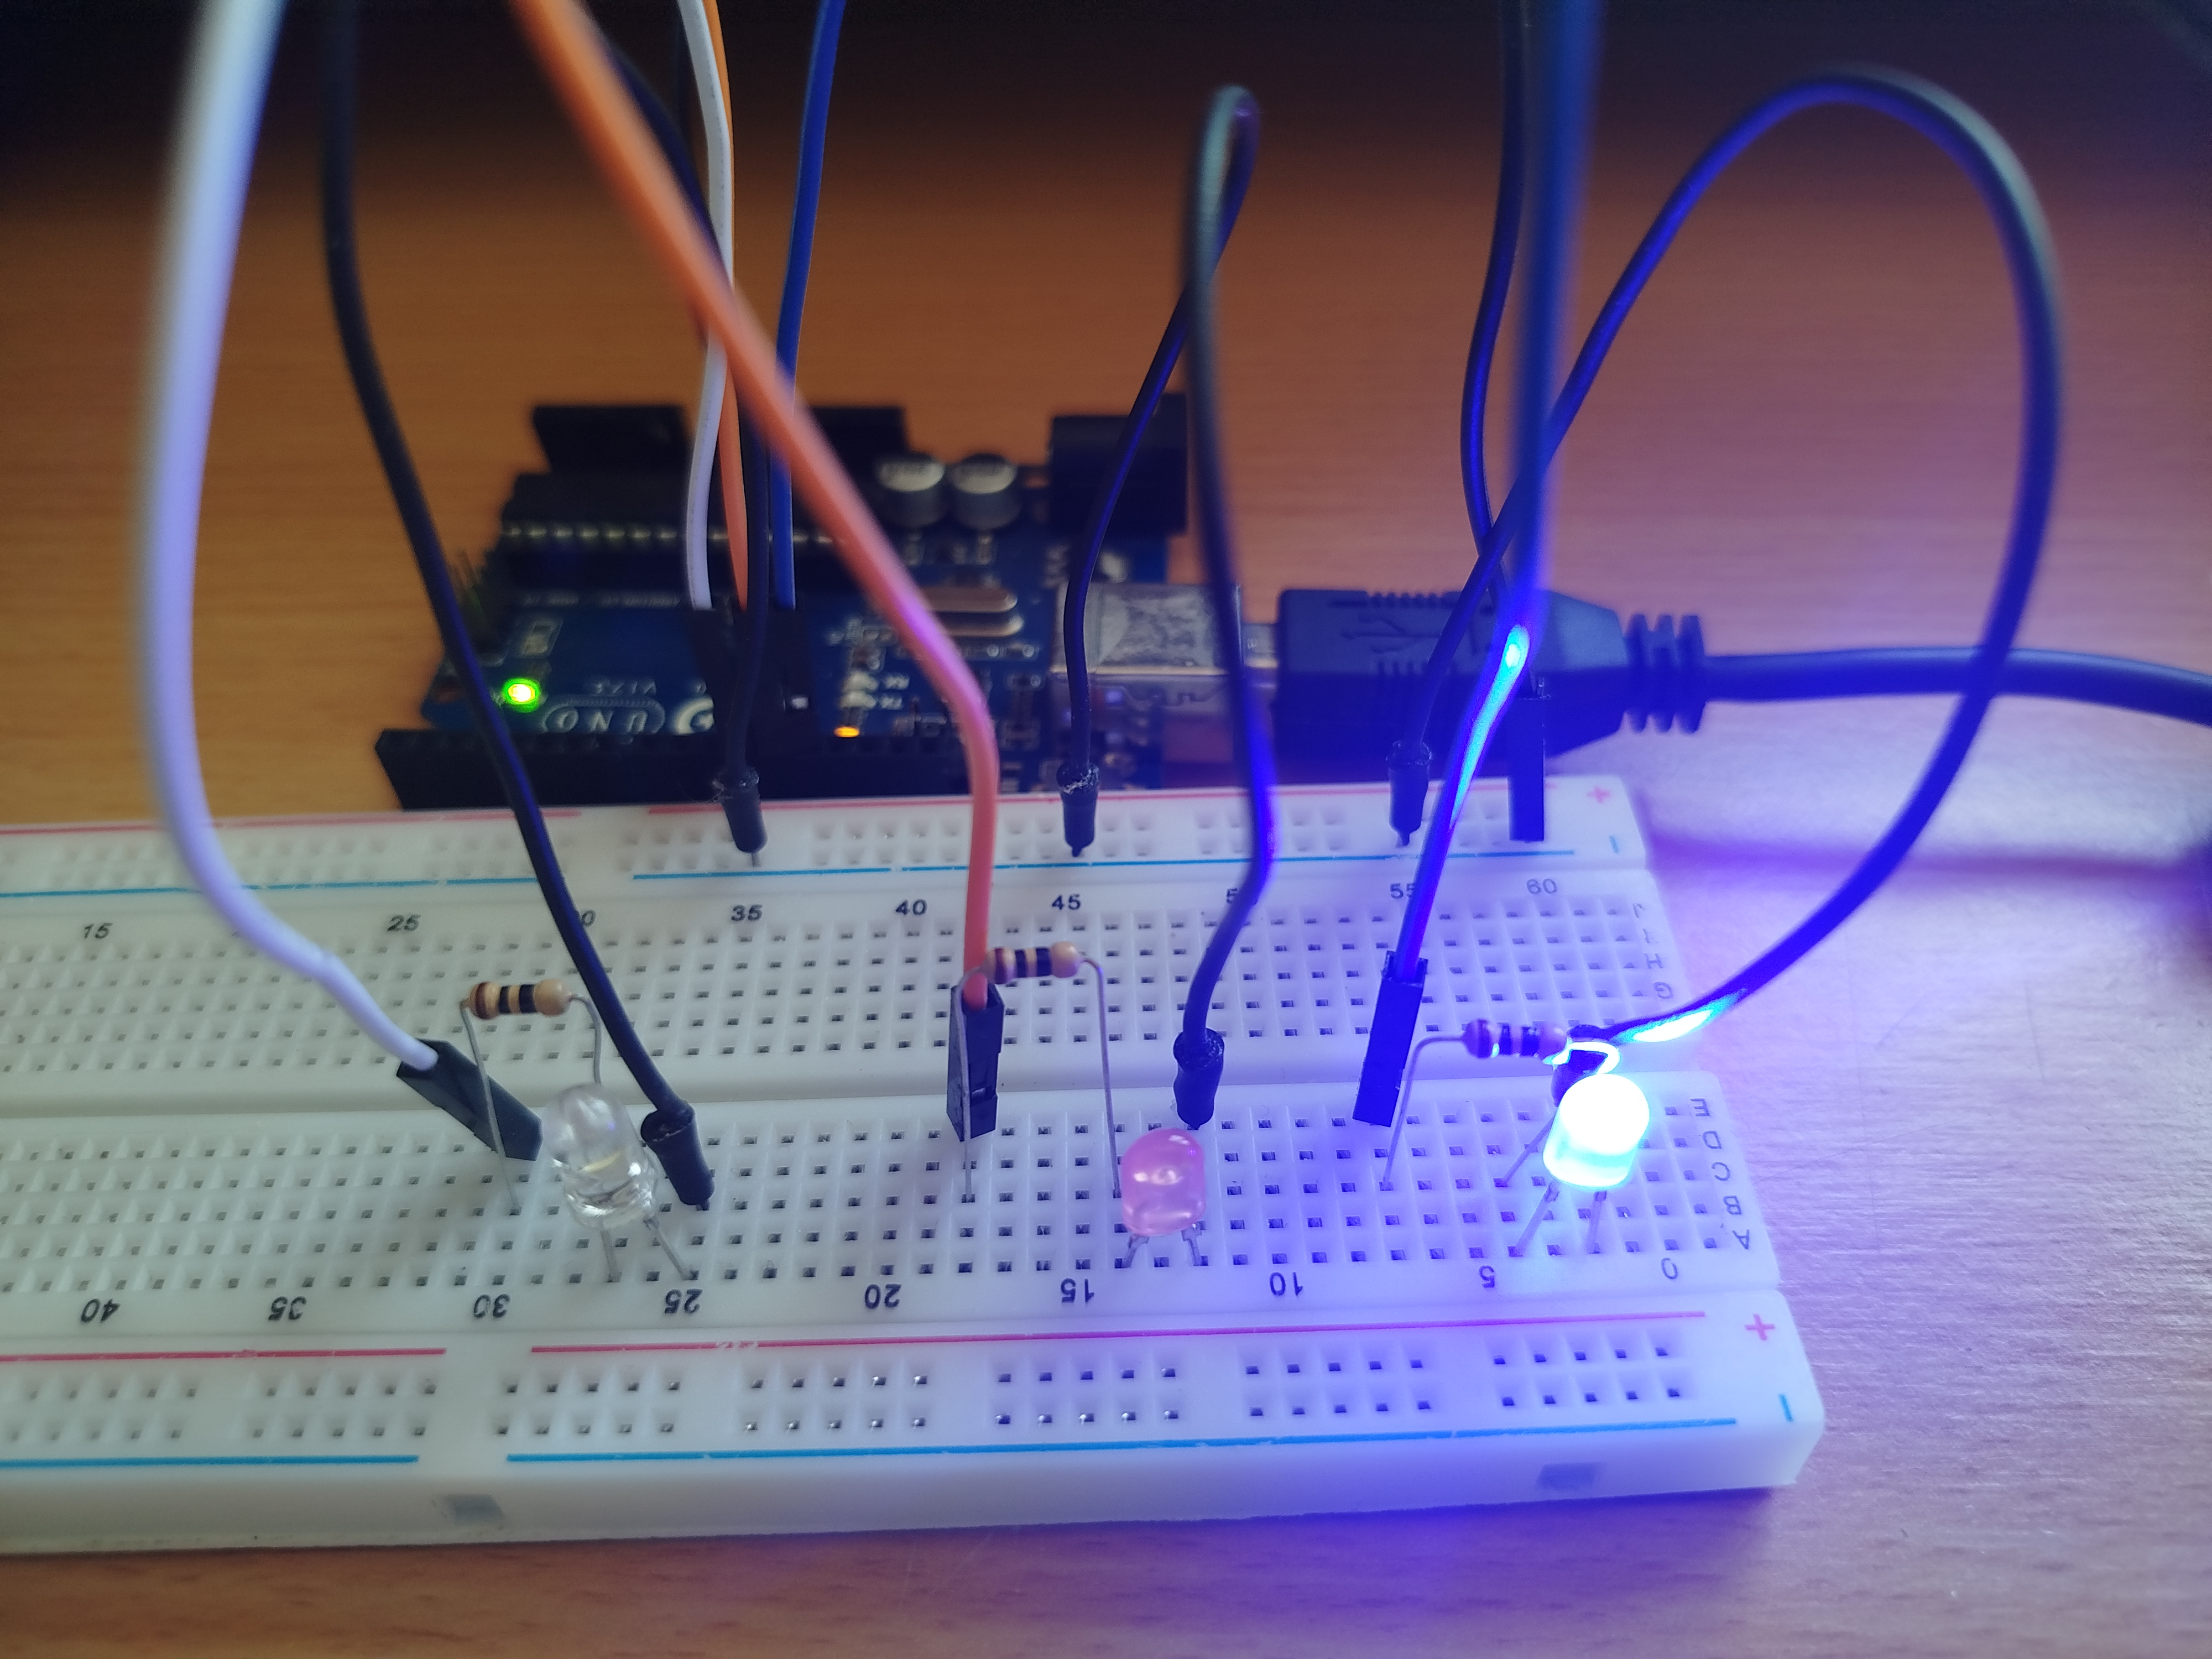
\includegraphics[width=0.6\textwidth]{images/img-3.jpg}
	\end{center}
	
	\section{Conclusion}
	This project demonstrates basic sequential digital output control using Arduino.
	It can be extended for more complex embedded systems.
	
\end{document}